\documentclass{mwhittaker}
\title{Bipartisan Paxos}

\usepackage{pervasives}
\usepackage{tikz}
\usetikzlibrary{calc}
\usetikzlibrary{positioning}
\usetikzlibrary{shapes.misc}

\begin{document}
\maketitle

\section{Overview}
Egalitarian Paxos~\cite{moraru2013there}, or EPaxos, is a state machine
replication protocol, like Raft~\cite{ongaro2014search} or Viewstamped
Replication~\cite{liskov2012viewstamped}. An EPaxos instance consists of a
fixed set of $n = 2f + 1$ nodes, where $f$ denotes the maximum allowable number
of node failures. With EPaxos, clients forward state machine commands to one of
the $n$ nodes. When a node receives a command $a$ from a client, it can get the
command $a$ chosen after one round trip of communication to a superquorum of
the $n$ nodes if no other concurrently proposed command conflicts with $a$. If
there is a concurrently proposed command that conflicts with $a$, then the node
can get $a$ chosen after potentially one additional round trip of communication
to a quorum (just a quorum, not a superquorum) of the $n$ nodes.

EPaxos has a number of nice features that set it apart from other state machine
replication protocols. For example, it can choose non-conflicting commands in
one round trip, disjoint sets of conflicting commands do not affect each other,
and superquorum sizes are one node smaller than the superquorum sizes used by
other protocols. The only bad thing about EPaxos is its complexity. It's not
easy to understand why EPaxos is correct.
%
In this paper, we describe a slight variant of EPaxos called Bipartisan Paxos,
or BPaxos. BPaxos retains almost all of the nice properties of EPaxos (BPaxos'
superquorum size is one larger than that of EPaxos) but is simpler to
understand.

\section{Bipartisan Paxos}
In this section, we describe BPaxos. We initially describe BPaxos as a simple
protocol that is very easy to understand, but not at all efficient. We then
repeatedly tweak the protocol. Every tweak makes the protocol more efficient,
and the tweaks also preserve the correctness of the protocol in a (hopefully)
obvious way. When we're finished tweaking, we end up with a protocol that has
almost the same performance guarantees as EPaxos.
%
We'll also warn you right now that we assume you have a good understanding of
Fast Paxos~\cite{lamport2006fast}. If you don't, the tweaks are not going to
make any sense.

\subsection{A Simple Protocol}
Recall that the EPaxos protocol is divided into two main components. The first
component constructs a directed graph of state machine commands and decides
when certain commands are considered \defword{committed}. The second component
executes the commands in reverse topological order one strongly connected
component at a time. BPaxos steals the second component, the command execution
component, from EPaxos without any modifications. The two algorithms execute
commands in 100\% the same way. Where BPaxos differs from EPaxos is in how it
constructs the graph and decides when commands in the graph are committed.

Our simple variant of BPaxos is illustrated in \figref{SimpleBPaxos}. A BPaxos
instance has three main components: an ordering service, a consensus service,
and a set of BPaxos nodes. We'll explain each of these three components
momentarily, but first we pause to review the notion of instances, borrowed
from EPaxos.

{\begin{figure}[ht]
  \centering

  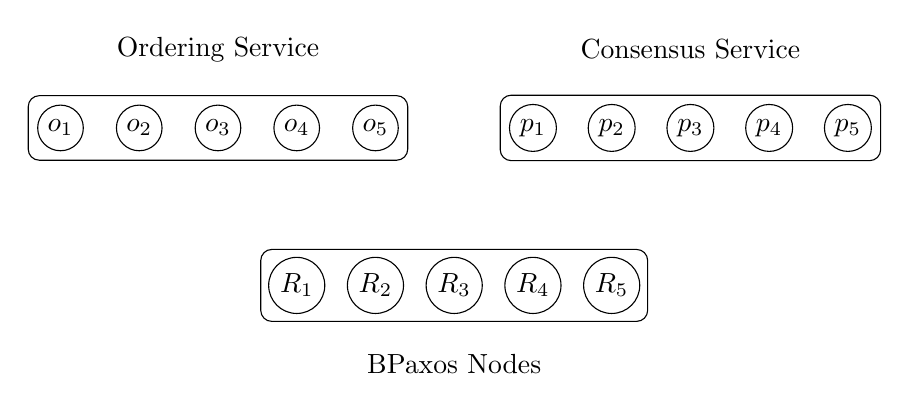
\begin{tikzpicture}
    \tikzstyle{machine}=[draw, circle, inner sep=2pt]

    % Ordering Service
    \node[machine] (o1) at (0, 2) {$o_1$};
    \node[machine] (o2) at (1, 2) {$o_2$};
    \node[machine] (o3) at (2, 2) {$o_3$};
    \node[machine] (o4) at (3, 2) {$o_4$};
    \node[machine] (o5) at (4, 2) {$o_5$};
    \node (os) at (2, 3) {Ordering Service};
    \draw[rounded corners]
      ($(o1.south west) + (-0.2, -0.2)$) rectangle
      ($(o5.north east) + (0.2, 0.2)$);

    % Consensus
    \node[machine] (p1) at (6, 2) {$p_1$};
    \node[machine] (p2) at (7, 2) {$p_2$};
    \node[machine] (p3) at (8, 2) {$p_3$};
    \node[machine] (p4) at (9, 2) {$p_4$};
    \node[machine] (p5) at (10, 2) {$p_5$};
    \node (os) at (8, 3) {Consensus Service};
    \draw[rounded corners]
      ($(p1.south west) + (-0.2, -0.2)$) rectangle
      ($(p5.north east) + (0.2, 0.2)$);

    % BPaxos Nodes
    \node[machine] (b1) at (3, 0) {$R_1$};
    \node[machine] (b2) at (4, 0) {$R_2$};
    \node[machine] (b3) at (5, 0) {$R_3$};
    \node[machine] (b4) at (6, 0) {$R_4$};
    \node[machine] (b5) at (7, 0) {$R_5$};
    \draw[rounded corners]
      ($(b1.south west) + (-0.2, -0.2)$) rectangle
      ($(b5.north east) + (0.2, 0.2)$);
    \node (bpaxos) at (5, -1) {BPaxos Nodes};
  \end{tikzpicture}

  \caption{Simple BPaxos}\figlabel{SimpleBPaxos}
\end{figure}
}

\paragraph{Instances}
As with EPaxos, every BPaxos node $R$ manages a set of numbered
\defword{instances} $R.1$, $R.2$, $R.3$, $\ldots$. As described in
\cite{moraru2013there}, we can visualize the set of instances as a
two-dimensional grid with the set of BPaxos nodes on the $x$-axis and the set
of instance numbers on the $y$-axis, as illustrated in
\figref{BPaxosInstances}.

{\begin{figure}[ht]
  \centering
  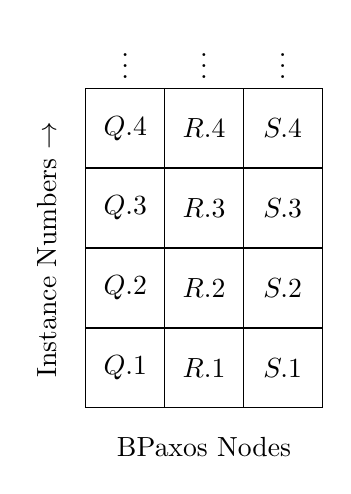
\begin{tikzpicture}
    \tikzstyle{box}=[draw, minimum width=1cm, minimum height=1cm]

    \node[box] (q1) at (0, 0) {$Q.1$};
    \node[box, above=0cm of q1] (q2) {$Q.2$};
    \node[box, above=0cm of q2] (q3) {$Q.3$};
    \node[box, above=0cm of q3] (q4) {$Q.4$};
    \node[above=0cm of q4] (qdots) {$\vdots$};

    \node[box] (r1) at (1, 0) {$R.1$};
    \node[box, above=0cm of r1] (r2) {$R.2$};
    \node[box, above=0cm of r2] (r3) {$R.3$};
    \node[box, above=0cm of r3] (r4) {$R.4$};
    \node[above=0cm of r4] (rdots) {$\vdots$};

    \node[box] (s1) at (2, 0) {$S.1$};
    \node[box, above=0cm of s1] (s2) {$S.2$};
    \node[box, above=0cm of s2] (s3) {$S.3$};
    \node[box, above=0cm of s3] (s4) {$S.4$};
    \node[above=0cm of s4] (sdots) {$\vdots$};

    \node (nodes) at (1, -1) {BPaxos Nodes};
    \node[rotate=90] (nodes) at (-1, 1.5) {Instance Numbers $\rightarrow$};
  \end{tikzpicture}
  \caption{BPaxos instances}%
  \figlabel{BPaxosInstances}
\end{figure}
}

\paragraph{Ordering Service}
\newcommand{\deps}[1]{\text{deps}(#1)}

On to the \defword{ordering service}. A BPaxos node $R$ sends a state machine
command $a$ to the ordering service for instance $R.i$. When the ordering
service receives a command $a$ for instance $R.i$, it replies with a tuple $(a,
\deps{a})$ where $a$ is the command and $\deps{a} = \set{I_1, \ldots, I_n}$ is
a set of instances that we call $a$'s \defword{dependencies}. The ordering
service provides the following guarantee. If two conflicting commands $a$ and
$b$ in instances $I_a$ and $I_b$ yield responses $(a, \deps{a})$ and $(b,
\deps{b})$ from the ordering service, then either $I_a \in \deps{b}$ or $I_b
\in \deps{a}$ (or both). That is, if two conflicting commands are sent to the
ordering service, at least one is guaranteed to be a dependency of the other.

Implementing a fault tolerant ordering service is straightforward. We employ
$2f + 1$ ordering service nodes $o_{1}, \ldots, o_{2f + 1}$. When a BPaxos node
$R$ sends a command $a$ in slot $R.i$ to the ordering service, it sends the
command to all $2f + 1$ of the ordering service nodes. Every ordering service
node $o_i$ maintains a set $O_i = {(c_1, I_1), (c_2, I_2), \ldots}$ of all the
commands and corresponding instances that it has received. When node $o_i$
receives a command $a$ for slot $I$ from a BPaxos node, it atomically performs
two actions.
%
First, $o_i$ replies to the BPaxos node with the pair $(a, \deps{a}_i)$ where
$\deps{a}_i = \setst{I}{\exists (c, I) \in O_i.\ \text{$a$ and $c$ conflict}}$
is the set of instances that $o_i$ has previously received that contain a
command that conflict with $a$.
%
Second, $o_i$ adds $a$ to $C_i$. When a BPaxos node receives replies $(a,
\deps{a}_{i_1}), \ldots, (a, \deps{a}_{i_{f+1}})$ from a quorum $Q_a$ of $f +
1$ ordering service nodes, it takes $(a, \deps{a}_{i_1} \cup \ldots \cup
\deps{a}_{i_{f+1}}) = (a, \deps{a})$ to be the response from the ordering
service.

To understand why this ordering service implementation provides its advertised
guarantees, consider conflicting commands $a$ and $b$ in instances $I_a$ and
$I_b$. Assume $a$'s reply $(a, \deps{a})$ was formed from a quorum $Q_a$ and
$b$'s reply $(b, \deps{b})$ was formed from a quorum $Q_b$. Any two quorums
intersect, so $Q_a \cap Q_b$ is nonempty. Let $o_i$ be an ordering service node
in this intersection. $o_i$ either received $a$ or $b$ first. If it received
$a$ first, then $(a, I_a)$ is in $O_i$ when $o_i$ processed command $b$, so
$o_i$ includes $I_a$ in $\deps{b}_i$, so $I_a$ is in $\deps{b}$. Symmetrically,
if $o_i$ received $b$ first, then it includes $I_b$ in $\deps{a}$.

\paragraph{Consensus Service}
Next up, the \defword{consensus service}. We assume we have some set $p_1,
\ldots, p_n$ of nodes that implement Plain Jane consensus. A BPaxos node can
propose to the consensus service that some value $v$ be chosen in some instance
$I$. The consensus service replies with the value that has been chosen in
instance $I$, which may or may not be $v$ depending on if there are concurrent
proposers proposing to instance $i$. The consensus service guarantees that for
every instance $i$, at most one value is ever chosen in $i$.

\paragraph{BPaxos Nodes}
Finally, we assume a fixed set $R_1, \ldots, R_{2f+1}$ of $2f + 1$ BPaxos
nodes.
%
Clients sends state machine commands to BPaxos nodes to be executed by the
replicated state machine. When a BPaxos node $R$ receives a command $a$, it
sends the command to the ordering service in a previously unused instance $R.i$
and receives a reply $(a, \deps{a})$. $R$ then proposes the value $(a,
\deps{a})$ to the consensus service in instance $R.i$. The consensus service
then replies with some chosen value $(a', \deps{a'})$, which is equal to $(a,
\deps{a})$ in the failure-free case. At this point, the command $a'$ is
considered committed in instance $R.i$ of the directed graph of state machine
commands with inbound edges from instances in $\deps{a'}$. Node $R$ also
informs the other BPaxos nodes that the value $(a', \deps{a'})$ has been
committed. As noted earlier, the execution of the commands in the directed
graph is identical to that of EPaxos. Committed commands are committed in
reverse topological order, one strongly connected component at a time.

\newcommand{\noop}{\text{noop}}
It's possible that (1) a committed command $a$ depends on an instance $R.i$
that contains an uncommitted command, and (2) the BPaxos node $R$ that manages
the instance $R.i$ has crashed. If the instance $R.i$ remains forever
uncommitted, then the command $a$ will never be executed. To avoid this
liveness violation, if any BPaxos node $S$ notices that instance $R.i$ has been
uncommitted for some time, it can propose to the consensus service that the
value $(\noop, \emptyset)$ be chosen in instance $R.i$ where $\noop$ is a
command that doesn't affect the state machine.

% TODO: Explain no liveness.

\paragraph{Correctness}
That's the basic version of BPaxos. We can prove it's correct by leveraging
EPaxos' proof of correctness. Open up \cite{moraru2013proof} and head to
section 5.6, which contains proofs of EPaxos' correctness.
\begin{itemize}
  \item
    \textbf{Theorem 1} says that EPaxos satisfies nontriviality. Clearly, so
    does BPaxos.

  \item
    \textbf{Lemma 1} says that EPaxos commits a command in an instance only if
    no other command will ever be committed in the same instance. The EPaxos
    proof is about two pages and not very easy to understand. However, the fact
    that BPaxos satisfies Lemma 1 is immediate from the fact that we use a
    consensus service. In fact, Lemma 1 is really just a restatement of the
    exact property that the consensus service provides.

  \item
    \textbf{Theorem 2} follows from Lemma 1.

  \item
    \textbf{Theorem 3} is trivial.

  \item
    \textbf{Theorem 4} states that if two conflicting commands are both
    committed, then they will be executed in the same order by every BPaxos
    node. The proof that BPaxos satisfies Theorem 4 is more or less the same as
    the proof that EPaxos satisfies theorem 4, which shouldn't be too
    surprising because BPaxos executes commands 100\% identically to EPaxos. In
    short, if two commands conflict, the ordering service guarantees that one
    will depend on the other. If both commands end up in the same strongly
    connected component, they will be executed in the same deterministic order.
    And, if the commands end up in different strongly connected components,
    then one component is guaranteed to be ordered before the other, so the two
    commands are executed in reverse topological order. There's also the
    wrinkle that we may commit a $\noop$, but $\noop$s don't conflict with any
    other commands, so we have nothing to worry about.
\end{itemize}

\subsection{Tweak 1: Colocation and Paxos}
For our first tweak, we'll do two things that don't actually improve the
performance of anything, but will set us up nicely for the following tweaks.
First, we choose to implement the consensus service with Paxos where the set
$p_1, \ldots, p_{2f+1}$ of consensus nodes are Paxos acceptors. We'll also
assume that every BPaxos node $R$ initially runs phase 1 of Paxos for every
instance $R.i$, the same trick played by Multi-Paxos. Second, we'll colocate
the ordering service nodes and the Paxos acceptors. We probably want to
colocate the BPaxos nodes with the ordering service nodes and Paxos acceptors
as well, but we won't show this in order to keep things simple.
%
The tweaked BPaxos architecture is illustrated in \figref{ColocatedBPaxos}.
Clearly, this tweak does not affect the correctness of our BPaxos protocol.

{\begin{figure}[ht]
  \centering

  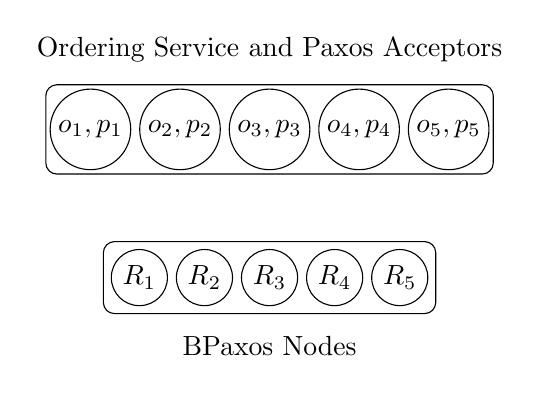
\begin{tikzpicture}
    \tikzstyle{machine}=[draw, circle, inner sep=2pt]

    % Ordering Service / Paxos Acceptors
    \node[machine] (o1) at (0, 2) {$o_1, p_1$};
    \node[machine, right=0.1cm of o1] (o2) {$o_2, p_2$};
    \node[machine, right=0.1cm of o2] (o3) {$o_3, p_3$};
    \node[machine, right=0.1cm of o3] (o4) {$o_4, p_4$};
    \node[machine, right=0.1cm of o4] (o5) {$o_5, p_5$};
    \node (os) at ($(o3.north) + (0, 0.5)$) {Ordering Service and Paxos Acceptors};
    \draw[rounded corners]
      ($(o1.south west) + (-0.2, -0.2)$) rectangle
      ($(o5.north east) + (0.2, 0.2)$);

    % BPaxos Nodes
    \node[machine, below=1cm of o3] (b3) {$R_3$};
    \node[machine, left=0.1cm of b3] (b2) {$R_2$};
    \node[machine, left=0.1cm of b2] (b1) {$R_1$};
    \node[machine, right=0.1cm of b3] (b4) {$R_4$};
    \node[machine, right=0.1cm of b4] (b5) {$R_5$};
    \draw[rounded corners]
      ($(b1.south west) + (-0.2, -0.2)$) rectangle
      ($(b5.north east) + (0.2, 0.2)$);
      \node (bpaxos) at ($(b3.south) + (0, -0.5)$) {BPaxos Nodes};
  \end{tikzpicture}

  \caption{Colocated BPaxos}\figlabel{ColocatedBPaxos}
\end{figure}
}

\subsection{Tweak 2: Fast Paxos}
Currently, the commit latency of BPaxos is two round trips in the normal case.
When a BPaxos node receives a command $a$ from a client, it (1) performs one
round trip to a quorum of ordering service nodes to obtain $(a, \deps{a})$, and
then (2) performs another round trip to a quorum of Paxos acceptors to have the
value $(a, \deps{a})$ chosen. Our second tweak will reduce the BPaxos commit
latency from two round trips (to two quorums) to one round trip (to a
superquorum). The idea behind the tweak is to implement our consensus service
using Fast Paxos instead of vanilla Paxos.

Upon initializing, every BPaxos node $R$ performs phase $1$ of Fast Paxos for
ballot $0$ for every Fast Paxos instance $R.i$. We let ballot $0$ be a fast
ballot, so after $R$ finishes executing phase 1, $R$ sends phase 2a ``any''
messages to the Fast Paxos acceptors. At this point, the acceptors are free to
vote for the first proposal that they hear from anyone (not just from $R$).

As before, when a BPaxos node $R$ receives a command $a$ from a client, it
sends the command to the ordering service nodes for some instance $R.i$.
Upon receiving $a$, the ordering service node $o_j$ computes its reply $(a,
\deps{a}_j)$. Now, here's the tweak. $o_j$ does not return the reply $(a,
\deps{a}_j)$ directly to $R$. Instead, it proposes the value $(a, \deps{a}_j)$
in instance $R.i$ to $p_j$ (the colocated Fast Paxos acceptor). As we just
described, $p_j$ votes for the first proposal that it hears from anyone, so
$p_j$ votes for the value $(a, \deps{a}_j)$ and relays its phase 2b vote back
to $R$.

If $R$ receives a superquorum of phase 2b votes for the same value $(a,
\deps{a}_{j_1}) = \cdots = (a, \deps{a}_{j_{m}})$ in instance $R.i$, then Fast
Paxos (and hence BPaxos) considers the value chosen. If $R$ does \emph{not}
receive a superquorum of phase 2b votes for the same value, then it computes
$(a, \deps{a})$ where $\deps{a}$ is the union of the dependencies in a quorum
of phase 2b votes. Then, it proposes the value $(a, \deps{a})$ be chosen in
$R.i$ with ballot $1$, a classic ballot, by running through the full two phases
of Paxos.

Thus, in the best case, BPaxos can commit a value in one round trip to a
superquorum. Note that this tweak really starts to emphasize the similarities
between BPaxos and EPaxos. EPaxos also commits a value in one round trip if it
hears back from a superquourm of nodes that all reply with identical values of
$(\gamma, seq_\gamma, deps_\gamma)$.

So why is this tweak correct? Well, first, we switched from using Paxos to
using Fast Paxos to implement our consensus service, but this change does not
affect correctness. Both protocols implement consensus, so it doesn't matter
which one we use. Second, consider when a BPaxos node $R$ receives a
superquorum of phase 2b votes for the same value $(a, \deps{a}_{j_1}) = \cdots
= (a, \deps{a}_{j_{m}})$. At this point, the value is chosen. But, this is
exactly what would have happened before this tweak as well. Before this tweak,
$R$ would have computed $(a, \deps{a})$ where $\deps{a} = \deps{a}_{j_1} \cup
\ldots \cup \deps{a}_{j_{m}}$, but $\deps{a}_{j_1} \cup \ldots \cup
\deps{a}_{j_{m}} = \deps{a}_{j_1} = \cdots = \deps{a}_{j_m}$! Thus, before the
tweak, $R$ would have attempted to get this value chosen anyway. This tweak
simply allows $R$ to avoid having to perform an extra round trip of
communication to get it chosen.

\subsection{Tweak 3: Coordinated Recovery}
After the previous tweak, a BPaxos node $R$ can commit a command in one round
trip if a superquorum of Paxos acceptors happen to vote for the same set of
dependencies. If $R$ does not receive a superquorum of matching votes, it
performs two additional phases of Paxos to get the command chosen in ballot 1.
Thus, we have one round trip commit latency in the best case and three round
trip commit latency in the next best case (and potentially infinitely more
round trips in the worst case~\cite{fischer1982impossibility}). This tweak, the
final tweak, improves BPaxos to one round trip commit latency in the best case
and two round trip commit latency in the next best case. This matches EPaxos'
commit latencies, save that BPaxos' superquorum sizes are one node larger.

The idea behind this tweak is to leverage a Fast Paxos feature called
coordinated recovery. Coordinated recovery says that if a Fast Paxos leader
owns consecutive ballots $i$ and $i + 1$, and hears phase 2b votes from a
quorum of acceptors for ballot $i$, it can skip phase 1 of ballot $i + 1$ and
proceed directly to phase 2. With this tweak, we make each BPaxos node the
leader of ballots $0$ and $1$. If BPaxos node $R$ receives a quorum of
non-equal votes in ballot $0$, it satisfies the conditions of coordinated
recovery and can initiate phase 2 of ballot 1 directly.

This tweak doesn't affect the correctness of BPaxos because it's merely a
performance optimization for Fast Paxos. The correctness of our protocol does
not depend on whether we use Paxos, Fast Paxos, or Fast Paxos with coordinated
recovery to implement our coordination service.

\section{Conclusion}
In summary, Bipartisan Paxos is a slight variant of Egalitarian Paxos that aims
to be more understandable at the cost of being slightly less performant. BPaxos
is easier to understand because it decomposes EPaxos into two decoupled
services---an ordering service and a consensus service---and then massages the
two together in an efficient way. BPaxos is less performant that EPaxos because
Fast Paxos superquorum sizes are one larger than EPaxos superquorum sizes.
Moreover, when a BPaxos node $R$ fails, other BPaxos nodes propose $\noop$s to
fill in any uncommitted instances of $R$. When an EPaxos node fails, other
EPaxos nodes have the ability to propose more than just $\noop$s.

\bibliographystyle{plain}
\bibliography{references}
\end{document}
